\chapter{Résultats et interprétations}

La perception sonore humaine est dite binaurale : c'est à dire qu'il y a deux «capteurs» (en l'occurence de chaque côté
de la tête).
Cette particularité est importante dans la perception de l'espace, en effet, le volume de la tête retarde la propagation
du son tout en déformant celui-ci permettant ainsi un repérage dans le plan horizontal (avec une précsion pouvant aller
jusqu'à un degré~\cite{Vor08}). Le torse a lui aussi une influence, particulièrement pour le répérage dans le plan
vertical. Au cours des mesures pour ce projet, une tête artificielle (sans torse) a été utilisée, le repérage vertical
sera donc difficile à reproduire d'après nos mesures.

\section{Essai 1 : une chanson en salle Mersenne} % {{{1

Le premier essai approfondi est réalisé en salle Mersenne. La source est au point \textbf{Source} (voir
figure~\ref{plan_mersenne}) et le recepteur au point \textbf{P1} (la tête est dans l'orientation par défaut).

\subsection{Comparaison perceptive} % {{{2

A l'écoute, la différence entre les deux résultats (monaural et binaural) est flagrante. Alors que la position de la
source est strictement indéterminable en monaural, elle est bien identifiable en binaural.

Des mesures plus précises auraient probablement permis une meilleure reconnaissance de la géométrie de la salle et des
obstacles, en particulier la paillasse présente sur la droite du récepteur.

\subsection{Comparaison fréquentielle} % {{{2

On note par ailleurs la différence de contenu fréquentiel (et en particulier la différence de niveau) sur la
figure~\ref{comp_mon_min_zoom_150_175}. Cette différence observée sur les spectres est bel et bien en accord avec la
comparaison perceptive menée ci-avant.
 On remarque que le signal monaural vient effectivement «s'intercaler» entre les
	2 canaux du signal binaural (en haut monaural et canal droit, en bas monaural et canal gauche). Une représentation
pleine échelle est disponible en annexe.


\begin{figure}[h!]
    \centering{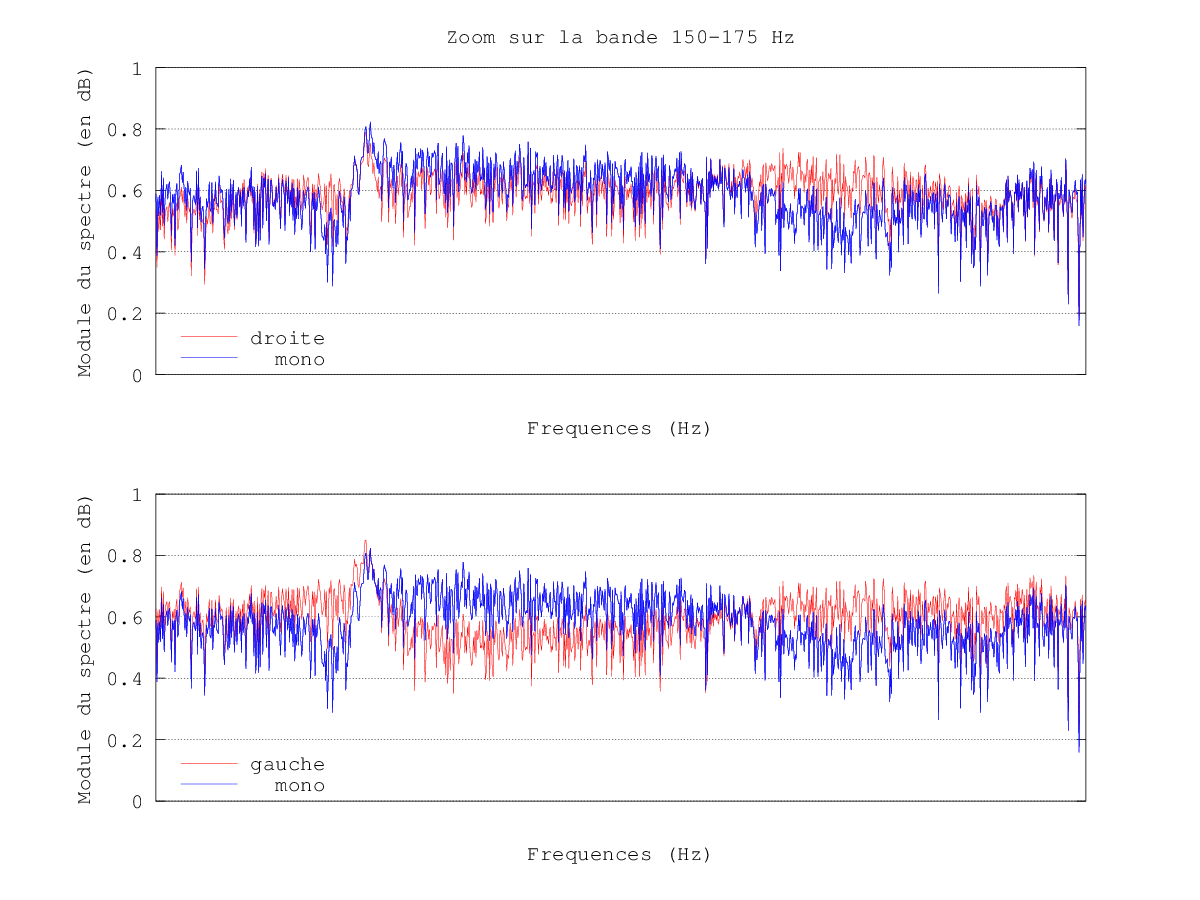
\includegraphics[width=13cm]{comp_mon_min_zoom_150_175.png}}
	\caption{\label{comp_mon_min_zoom_150_175}Comparaison entre les contenus fréquentiels des signaux monaural et
	binaural dans la bande 150-175Hz.}
\end{figure}

\newpage % MISE EN PAGE

\subsection{Comparaison temporelle} % {{{2 


\begin{figure}[h!]
    \centering{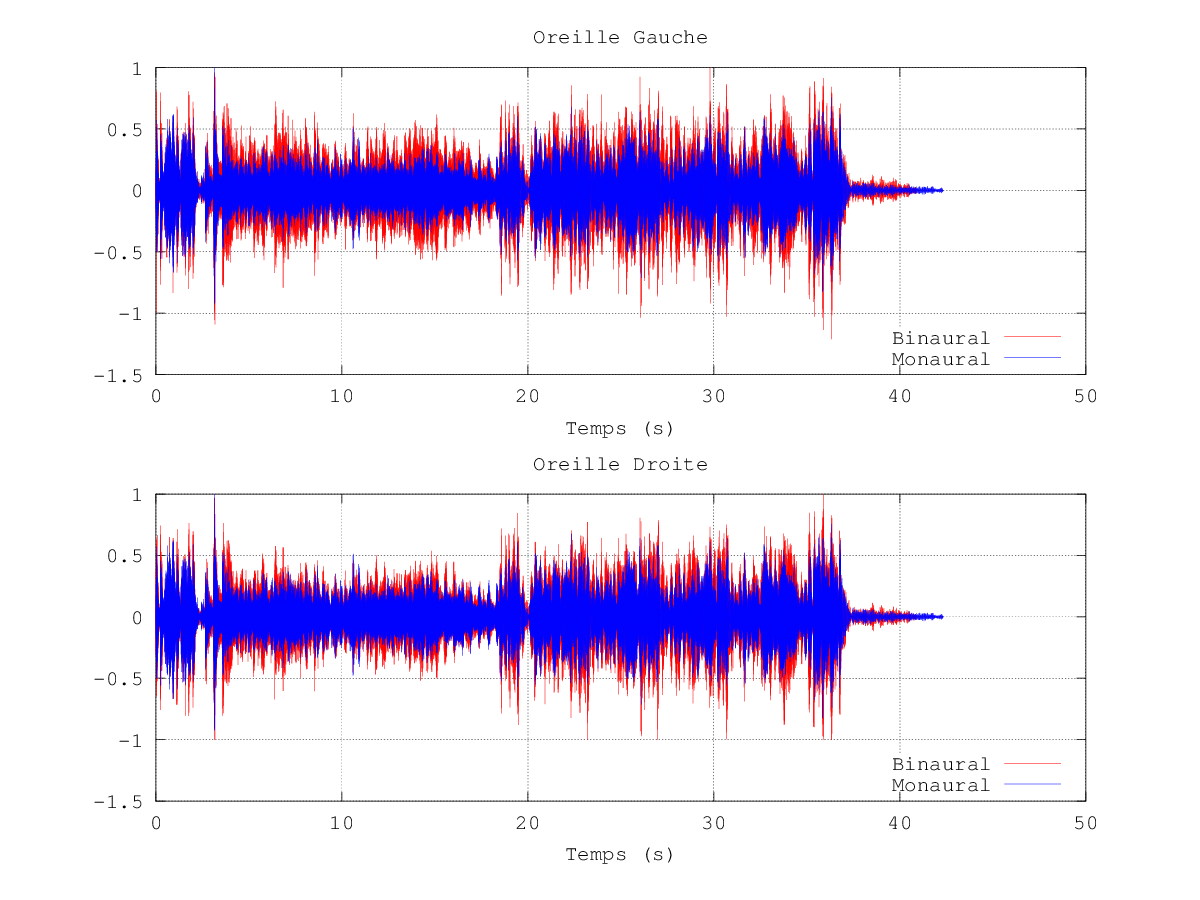
\includegraphics[width=13cm]{temporel_cale.png}}
    \caption{\label{comp_mon_bin_P1_enveloppe}}Tracés temporels des signaux convolués pour une RI monaurale (en bleu) et
    une RI binaurale en rouge. En haut pour l'oreille gauche et en bas pour l'oreille droite.}
\end{figure}

La figure~\ref{comp_mon_bin_P1_enveloppe} montre les tracés temporels des signaux convolués en monaural et binaural.
Les différences sont assez minimes (mise à part l'amplitude). Les enveloppes sont très ressemblantes. Un même son est
convolué à chaque fois, le résultat est donc censé être ressemblant.

\section{Essai 2 : des claquements de mains en salle réverbérante} % {{{1

Un autre essai est mené en salle réverbérante. Il s'agit cette fois de vérifier que les différentes réflexions sont
correctement restituées lors de la convolution.

\subsection{Comparaison temporelle} % {{{2

\begin{figure}[h!]
    \centering{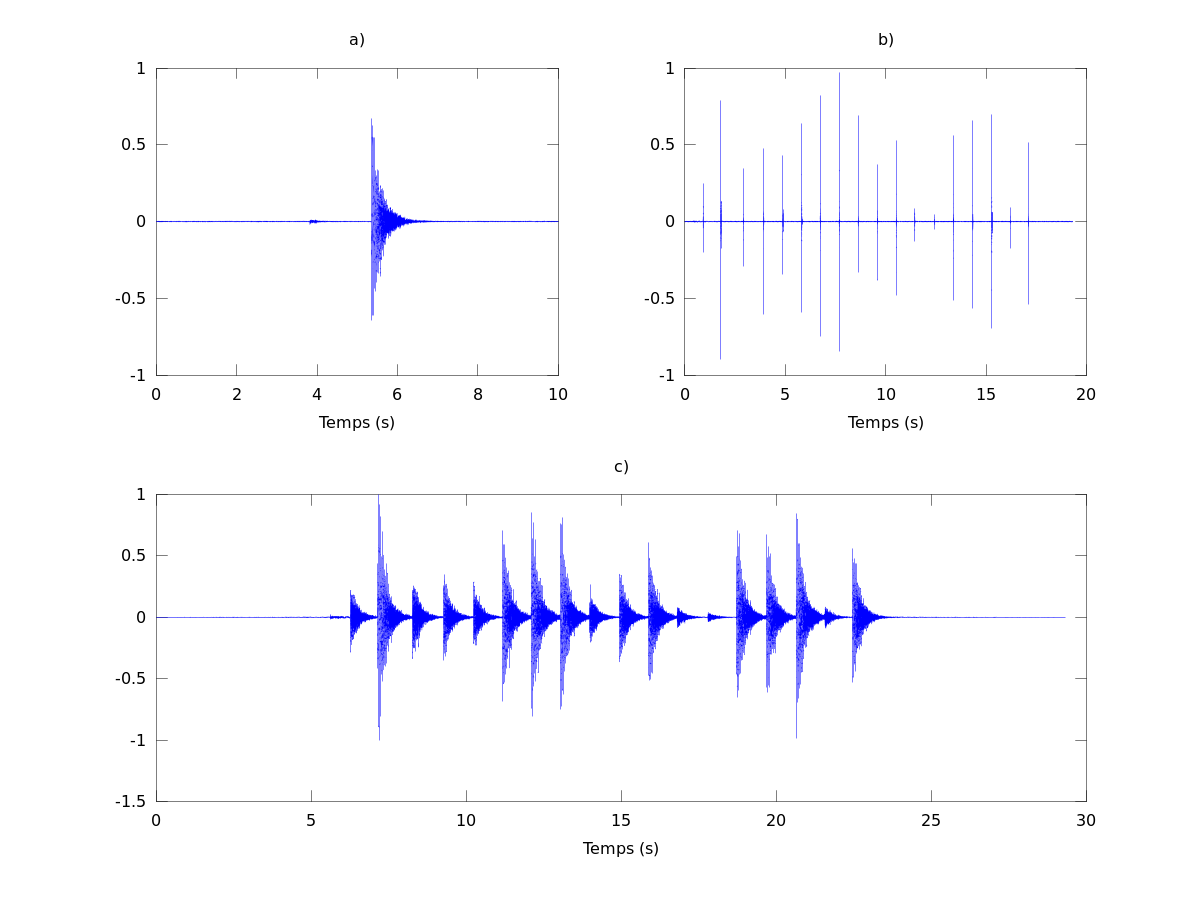
\includegraphics[width=13cm]{temporel_reverb.png}}
	\caption{\label{temporel_reverb}Tracé des différents signaux et résultat de la convolution en temporel. En a) la
    RI utilisée, en b) le son anéchoïque, en c) le résultat après convolution des deux signaux précédents.}
\end{figure}

La figure~\ref{temporel_reverb} montre les différents signaux utilisés et leur convolution. Ici, le résultat est donné
en monaural, on note que les réflexions visibles sur la RI sont clairement restituées sur le signal final.

En binaural, le résultat de chaque canal ressemble très fortement au résultat en monoral présenté ci-avant.

\subsection{Comparaison perceptive} % {{{2

L'écoute se fait sur les convolutions binaurales.

Perceptivement, le résultat est probant. L'influence de la salle réverbérante s'entend très bien et l'immersion se fait
sans souci.

La provenance du son est moins clairement identifiable que pour une salle plus matte (salle Mersenne par exemple),
mais toujours nettement plus identifiable qu'en monaural.

\section{Ecoute par d'autres personnes} % {{{1

Tout au long du projet, les sons résultants ont été écoutés par plusieurs personnes étrangères au projet.

Il ressort plusieurs choses de ces écoutes :

\begin{itemize}
    \item tous trouvent le résultat étonnant ;
    \item la plupart (presque tous) réussit à retrouver la provenance du son lors d'écoutes de résultats binauraux ;
    \item les écoutes monaurales sont troublantes pour ceux les écoutent (incapacité à localiser la source, symétrie 
    auditive inhabituelle) ;
    \item ceux connaissant la différence entre salle mate et salle réverbérante lient clairement les écoutes aux types
    de salles, les autres parlent de \textit{«plus de reverb»} pour les résultats utilisant une salle réverbérante ;
    \item les résultats liés à la salle Mersenne donnent à certains l'impression que ce qu'ils entendent provient de la
    salle où ils se trouvent et non du casque.
\end{itemize}

Finalement, la qualité des écouteurs utilisés influe grandement sur le résultat. L'immersion est assez faible pour de
simple écouteurs, elle demande une certaine concentration. En utilisant des écouteurs intra-auriculaires, l'immersion
est largement meilleure et la provenance est plus facilement identifiable. Les sons semblent plus naturels. Les
meilleurs résultats sont obtenus en utilisant un casque isolant convenablement l'auditeur des bruits qui l'entourent.
L'immersion est alors bonne.
